\RequirePackage{plautopatch}
\RequirePackage[l2tabu, orthodox]{nag}

\documentclass[dvipdfmx]{jlreq}
\usepackage{graphicx}
\usepackage{natbib}
\usepackage{hyperref}
\usepackage{amsmath}
\usepackage{amssymb}
\usepackage{lscape}
\usepackage{pdflscape}

\usepackage{listings}
\usepackage{xcolor}

\lstset{
  basicstyle={\ttfamily},
  identifierstyle={\small},
  commentstyle={\small\itshape},
  keywordstyle={\small\bfseries},
  ndkeywordstyle={\small},
  stringstyle={\small\ttfamily},
  frame={tb},
  breaklines=true,
  columns=[l]{fullflexible},
  numbers=left,
  xrightmargin=0zw,
  xleftmargin=3zw,
  numberstyle={\scriptsize},
  stepnumber=1,
  numbersep=1zw,
  lineskip=-0.5ex
}


\title{
\vspace{-4cm}
モデルの修正（ディスカッション）
}

\author{岸本康佑}
\date{2026年5月27日}

\begin{document}
\maketitle
\tableofcontents

%本文開始
\section{Farmer}
Farmerの行動は以下の効用最大化問題の解として定式化できる
\begin{align}
  \max_{x_t, b_t, k_t, q_t} \quad & \mathbb{E}_t \bigg( \sum_{s=0}^{\infty} \beta^s x_{t+s} \bigg) \label{eq:f_u} \\
  \text{s.t.} \quad & q_t(k_t - k_{t-1}) + R b_{t-1} + x_t - c k_{t-1} = a k_{t-1} + b_t \label{eq:f_yosan} \\
  & R b_t \leq q_{t+1} k_t \label{eq:kariire}\\
  & x_t \geq c k_{t-1} \label{eq:syouhi}
\end{align}

\begin{itemize}
  \item \eqref{eq:f_u}式は，消費$x_t$の割引現在価値の合計であり，Farmerの効用関数
  \item \eqref{eq:f_yosan}式は，左辺第1項が不動産購入費用，第2項が借入金の返済，$x_t-ck_{t-1}$が自家消費分の生産を超えた消費，右辺が生産と借入による収入を表す予算制約式
  \item \eqref{eq:kariire}式は不動産価値$q_{t+1} k_t$を超えて，金利を含めた借入$R b_t$ができないという借入制約
  \item \eqref{eq:syouhi}式はnot-tradable output以上の消費$x_t$をするという消費制約
\end{itemize}

\subsection{Farmerの最適化}
Farmerの効用最大化問題のラグランジアンは以下の通り
\begin{equation}
  \begin{aligned}
    \mathcal{L} = \mathbb{E}_0 \sum_{s=0}^{\infty} \beta^s \bigg[ & x_{t+s} + \lambda_{t+s} [(a + c) k_{t+s-1} + b_{t+s} - q_{t+s} (k_{t+s} - k_{t+s-1}) \\
    &- R b_{t+s-1} - x_{t+s}] \\
    &+\mu_{t+s}[q_{t+s+1}k_{t+s} - R b_{t+s}] + \varphi_{t+s}[x_{t+s} - ck_{t+s-1}] \bigg]
  \end{aligned}
\end{equation}

効用最大化の1階条件を導出する
\begin{align}
  &\frac{\partial\mathcal{L}}{\partial x_t}: 1 - \lambda_t + \varphi_t = 0 \\
  &\frac{\partial\mathcal{L}}{\partial b_t}: \lambda_t - \mu_t R - \beta \lambda_{t+1} R = 0 \\
  &\frac{\partial\mathcal{L}}{\partial k_t}: - q_t \lambda_t + \mu_t q_{t+1} + \beta \lambda_{t+1}[(a+c) + q_{t+1}] - \beta c \varphi_{t+1} = 0
\end{align}  

上記の1階条件より，自家消費制約と不動産価格のオイラー方程式を得る
\begin{align}
  1 + \varphi_t &= (\beta(1+\varphi_{t+1}) + \mu_t) R \\
  q_t (1 + \varphi_t) + \beta c \varphi_{t+1} &= \beta(1 + \varphi_{t+1})[a + c + q_{t+1}] + \mu_t q_{t+1} \label{eq:f_land}
\end{align}

\newpage

\section{Gatherer}
Gahtererの行動は以下の効用最大化問題の解として定式化できる
\begin{align}
  \max_{x'_t, b'_t, k'_t, q_t} \quad & \mathbb{E}_t \bigg( \sum_{s=0}^{\infty} \beta'^s x'_{t+s} \bigg) \label{eq:g_u} \\
\text{s.t.} \quad & q_t(k'_t - k'_{t-1}) + R b'_{t-1} + x'_t = G(k'_{t-1}) + b'_t \label{eq:g_yosan}
\end{align}

\begin{itemize}
  \item \eqref{eq:g_u}式は，消費$x'_t$の割引現在価値の合計であり，Gathererの効用関数
  \item \eqref{eq:g_yosan}式は，左辺第1項が不動産購入費用，第2項が借入の返済，第3項が消費，右辺が生産と借入による収入を表す予算制約式
  \item 定常状態では，Gathererは貸し手側なので$b'_t < 0$，すなわち左辺第2項は貸した資金の返済である
\end{itemize}

\subsection{Gathererの最適化}
Gathererの効用最大化問題のラグランジアンは以下の通り
\begin{equation}
  \begin{aligned}
    \mathcal{L} = \mathbb{E}_0 \sum_{s=0}^{\infty} \beta'^s \bigg[ & x'_{t+s} + \lambda'_{t+s} [G(k'_{t+s-1}) + b'_{t+s} - q_{t+s} (k'_{t+s} - k'_{t+s-1} - R b'_{t+s-1} - x'_{t+s}] \bigg]
  \end{aligned}
\end{equation}

効用最大化の1階条件を導出する
\begin{align}
  \frac{\partial \mathcal{L}}{\partial x_t'} &: 1 - \lambda_t' = 0 \\
  \frac{\partial \mathcal{L}}{\partial b_t'} &: \lambda_t' - \beta' R_t \lambda_{t+1}' = 0 \\
  \frac{\partial \mathcal{L}}{\partial k_t'} &: -\lambda_t' q_t + \beta \lambda_{t+1}' G'(k_t') + \beta q_{t+1} = 0
\end{align}

名目金利$R$の定義式と不動産価格$q_t$のオイラー方程式を得る
\begin{align}
  1 &= \beta' R \\
  q_t &= \beta' [G'(k'_t) + q_{t+1}]
\end{align}

\newpage

\section{モデルの全体像}
\begin{gather}
  q_t(k_t - k_{t-1}) + \frac{1}{\beta'} b_{t-1} + x_t - c k_{t-1} = a k_{t-1} + b_t \\
  b_t \leq \beta' q_{t+1} k_t \\
  x_t \geq c k_{t-1} \\
  1 + \varphi_t = (\beta(1+\varphi_{t+1}) + \mu_t) \frac{1}{\beta'} \label{} \\
  q_t (1 + \varphi_t) + \beta c \varphi_{t+1} = \beta(1 + \varphi_{t+1})[a + c + q_{t+1}] + \mu_t q_{t+1} \\
  q_t = \beta' [G'(k'_t) + q_{t+1}] \\
  x_t + m x'_t = (a + c) k_{t-1} + m G(k'_{t-1}) \label{eq:kinkou1} \\
  k_t + m k'_t = \bar{K} \label{eq:kinkou2}
\end{gather}
8本の方程式，8個の変数，6個のパラメータを持つKiyotaki-Mooreモデルが導出された．

ただし，
\begin{equation}
  b_t + m b'_t = 0
\end{equation}
とし，\eqref{eq:kinkou1}式は総生産量であり$Y_t$とおく．
また$\bar{K}$は定数である．\eqref{eq:kinkou1}式，\eqref{eq:kinkou2}式は均衡条件式である．

\begin{itemize}
  \item \textbf{変数} \\
    $k$：Farmerが保有する不動産，$k'$：Gathererが保有する不動産， \\
    $x$：Farmerの消費，$x'$：Gathererの消費， \\
    $ak$：Farmerの取引可能な生産物，$ck$：Gathererの取引不可能だが自家消費可能な生産物， \\
    $b$：Farmerの借入金（Gathererの貸出金），$q$：不動産価格
  \item \textbf{関数} \\
    $G(k')$：Gathererの生産関数（分析では$G(k')=(z+k')^\alpha$のコブ・ダグラス型）
  \item \textbf{パラメータ} \\
    $\beta$：Farmerの割引率，$\beta'$：Gathererの割引率
  \item \textbf{定数} \\
    $\bar{K}$：不動産の総量，$m$：FarmerとGatherの割合
  \item \textbf{ラグランジュ乗数} \\
    $\mu$：借入制約，$\varphi$：自家消費制約
\end{itemize}
※ダッシュ記号「'」が付いているものはGatherer関連である．

\newpage

\section{総量規制ショックの追加（借入制約に対するショック）}
Farmerの借入制約$R b_t \leq q_{t+1} k_t$にショック項$\varepsilon_t$を加えると，
\begin{equation}
  R b_t \leq q_{t+1} k_t (1+\varepsilon_t)
\end{equation}
となる．よって，Farmerの効用最大化問題のラグランジアンは，
\begin{equation}
  \begin{aligned}
    \mathcal{L} = \mathbb{E}_0 \sum_{s=0}^{\infty} \beta^s \bigg[ & x_{t+s} + \lambda_{t+s} [(a + c) k_{t+s-1} + b_{t+s} - q_{t+s} (k_{t+s} - k_{t+s-1}) \\
    &- R b_{t+s-1} - x_{t+s}] \\
    &+\mu_{t+s}[q_{t+s+1}k_{t+s}(1+\varepsilon_t) - R b_{t+s}] + \varphi_{t+s}[x_{t+s} - ck_{t+s-1}] \bigg]
  \end{aligned}
\end{equation}
だから，効用最大化の1階条件より，
\begin{align}
  &\frac{\partial\mathcal{L}}{\partial x_t}: 1 - \lambda_t + \varphi_t = 0 \\
  &\frac{\partial\mathcal{L}}{\partial k_t}: - q_t \lambda_t + \mu_t q_{t+1}(1+\varepsilon_t) + \beta \lambda_{t+1}[(a+c) + q_{t+1}] - \beta c \varphi_{t+1} = 0
\end{align}
よって，Farmerの不動産価格のオイラー方程式は，
\begin{equation}
  q_t (1 + \varphi_t) + \beta c \varphi_{t+1} = \beta (1 + \varphi_{t+1})[a + c + q_{t+1}] + \mu_t q_{t+1} (1+\varepsilon_t)
\end{equation}
に変わる．

よって，ショック項を含めたモデルの全体像は，
\begin{gather}
  q_t(k_t - k_{t-1}) + \frac{1}{\beta'} b_{t-1} + x_t - c k_{t-1} = a k_{t-1} + b_t \label{eq:b_model1} \\
  b_t \leq \beta' q_{t+1} k_t (1+\varepsilon_t) \label{eq:b_model2} \\
  x_t \geq c k_{t-1} \\
  1 + \varphi_t = (\beta(1+\varphi_{t+1}) + \mu_t) \frac{1}{\beta'} \label{} \\
  q_t (1 + \varphi_t) + \beta c \varphi_{t+1} = \beta(1 + \varphi_{t+1})[a + c + q_{t+1}] + \mu_t q_{t+1} (1+\varepsilon_t) \label{eq:b_model5} \\
  q_t = \beta' [G'(k'_t) + q_{t+1}] \label{eq:b_model6} \\
  x_t + m x'_t = (a + c) k_{t-1} + m G(k'_{t-1}) \label{eq:b_model7} \\
  k_t + m k'_t = \bar{K} \label{eq:b_model8}
\end{gather}
となる．

パラメータの値を$\beta=0.98, \beta'=0.99, a=0.7, c=0.3, \alpha=1/3, m=0.5, \bar{K}=1, z=0.01$と仮置きしてシミュレーションした結果が図\ref{fig:b}である．

\newpage

\begin{landscape}
  \begin{figure}
    \centering
    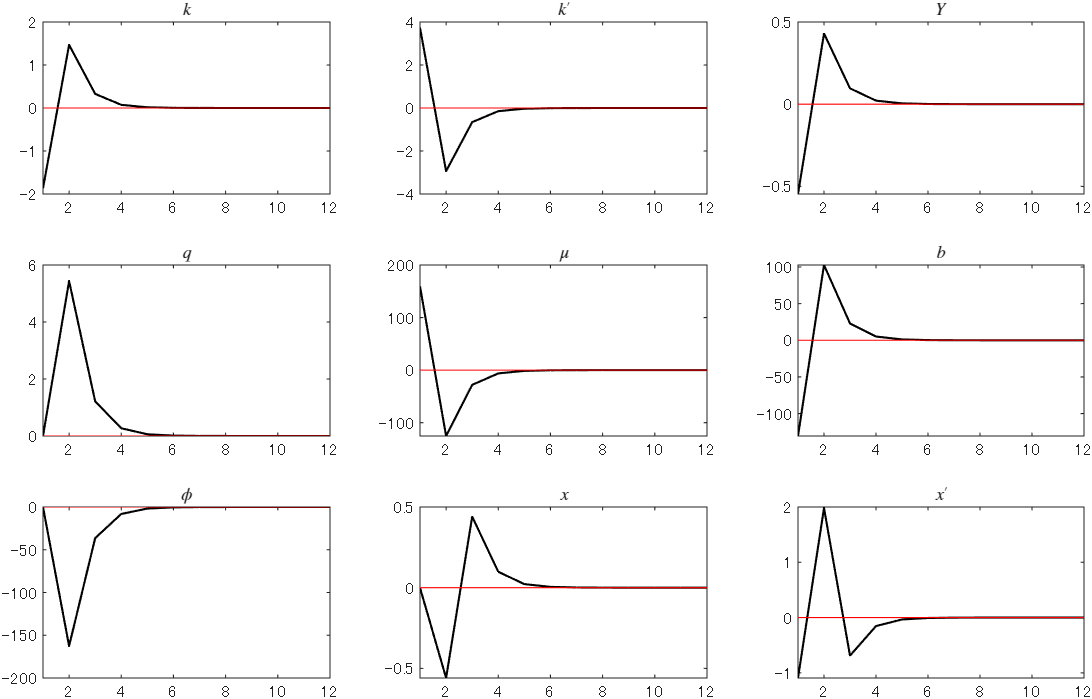
\includegraphics[scale=1.3]{b.png}
    \caption{借入制約へのショック}
    \label{fig:b}
  \end{figure}
\end{landscape}

\newpage

\subsection{考察}
\begin{itemize}
  \item \textbf{借入金$b$は1期目で減少し，2期目で増加．その後も増加を続け5期目で収束}
  \begin{itemize}
    \item 1期目の減少はショックの直接的な影響（∵借入制約式（\eqref{eq:b_model2}式））
    \item 2期目の増加は，Farmerの不動産の新規購入$q_t(k_t - k_{t-1})$と，Farmerの1期目の生産$(a+c)k_{t-1}$の増加が影響（∵Farmerの予算制約式（\eqref{eq:b_model1}式））
    \item $k_t - k_{t-1}$が負，Farmerの生産$(a+c)k_{t-1}$の増加が影響して，定常状態に収束（∵Farmerの予算制約式）
  \end{itemize}
\end{itemize}

\begin{itemize}
  \item \textbf{Farmerの不動産保有$k$は1期目で減少し，2期目で増加．その後も増加を続け5期目で収束}
  \begin{itemize}
    \item 1期目の減少はショックの直接的な影響（∵借入制約式）
    \item 2期目以降は借入金$b$の増加や，借入金の返済$\frac{1}{\beta'} b_{t-1}$の減少によって不動産保有を増やす（∵Farmerの予算制約式）
    \item Gathererの不動産保有$k'$は$k$の動きと逆の動きをする（∵不動産の量は一定（\eqref{eq:b_model8}式））
  \end{itemize}
\end{itemize}


\begin{itemize}
  \item \textbf{総生産量$Y$は1期目で下がって，2期目で上昇．その後も上昇を続け5期目で収束}
  \begin{itemize}
    \item FarmerとGatherの両方で生産が行われているので，パラメータの値によって増加する場合もある（∵総生産量の定義式（\eqref{eq:b_model7}式））
  \end{itemize}
\end{itemize}

\begin{itemize}
  \item \textbf{不動産価格$q$は2期目をピークに一貫して上昇．5期目に収束}
  \begin{itemize}
    \item Gathererの不動産保有$k'$が増加し，不動産のファンダメンタルズ$G'(k')$が上昇（∵不動産のオイラー方程式（\eqref{eq:b_model6}式））
    \item ピークや増加のペースも$k'$の増加に対応
    \item Gathererの限界生産$G'(k')$は，$k'$が増加するにつれて減少するので，2期目をピークに下落
    \item 不動産価格のオイラー方程式（\eqref{eq:b_model5}式）にショック項を加えたので$q$を下げる効果があると予想したが，この項を除いても結果はほとんど変わらず
  \end{itemize}
\end{itemize}

総量規制ショックに対して，$q$が一貫して上昇しているのはVAR分析の結果と整合的でないため，モデルの修正が必要

\newpage

\section{モデルの修正案}
総量規制ショックに対して，$q$が下落するようにモデルの修正を試みる

\subsection{借入制約の$q_{t+1}$を$q_t$に変更} \label{q_change}
\begin{itemize}
  \item Kiyotaki-Mooreモデルでは不動産（原論文：土地）担保の価格を，担保を売ることになる来期の価格と想定していた
  \item ここでの変更は，バブル崩壊期のGatherer（資本家）は将来ではなく現時点での担保価格を参考に貸し出しを行っていたと想定するものである
  \item この想定は，バブル期以来，不動産価格が乱高下しており正確な将来予測ができなかったという背景から合理的である
  \item しかし，Dynareで計算を行った結果，Blanchard-Kahn条件（以下，BK条件）が満たされないことが分かった
  \item パラメータの値を仮置きしているので，変更すればBK条件を満たす可能性はある
  \item ただし，もし仮にBK条件が満たされるようなパラメータの値が分かったとしても，不動産価格のファンダメンタルズがGathererの限界生産であるという根本的な原因は解決できず，1期目の下落に留まる可能性がある
\end{itemize}

\subsection{Farmerの生産関数を$(a+c)k^\theta$に変更} \label{product_change}
\begin{itemize}
  \item 生産関数を$(a+c)k^\theta$にすることで，不動産価格のオイラー方程式（\eqref{eq:b_model5}式）にFarmerの限界生産をファンダメンタルズとして導入することが可能である
  \item これにより，Gathererの不動産保有の増加による$q$の上昇（\eqref{eq:b_model6}式）と，Farmerの不動産保有の減少による$q$の下落の両方を表現でき，パラメータの値によって$q$の下落効果を大きくすることができる可能性がある
\end{itemize}

Farmerの効用最大化問題を定式化し直すと，
\begin{align}
  \max_{x_t, b_t, k_t, q_t} \quad & \mathbb{E}_t \bigg( \sum_{s=0}^{\infty} \beta^s x_{t+s} \bigg) \\
  \text{s.t.} \quad & q_t(k_t - k_{t-1}) + R b_{t-1} + x_t - c k_{t-1}^\theta = a k_{t-1}^\theta + b_t \\
  & R b_t \leq q_{t+1} k_t \\
  & x_t \geq c k_{t-1}^\theta
\end{align}

ラグランジアンは，
\begin{equation}
  \begin{aligned}
    \mathcal{L} = \mathbb{E}_0 \sum_{s=0}^{\infty} \beta^s \bigg[ & x_{t+s} + \lambda_{t+s} [(a + c) k_{t+s-1}^\theta + b_{t+s} - q_{t+s} (k_{t+s} - k_{t+s-1}) \\
    &- R b_{t+s-1} - x_{t+s}] \\
    &+\mu_{t+s}[q_{t+s+1}k_{t+s} - R b_{t+s}] + \varphi_{t+s}[x_{t+s} - ck_{t+s-1}^\theta] \bigg]
  \end{aligned}
\end{equation}

効用最大化の1階条件を導出する
\begin{align}
  &\frac{\partial\mathcal{L}}{\partial x_t}: 1 - \lambda_t + \varphi_t = 0 \\
  &\frac{\partial\mathcal{L}}{\partial b_t}: \lambda_t - \mu_t R - \beta \lambda_{t+1} R = 0 \\
  &\frac{\partial\mathcal{L}}{\partial k_t}: - q_t \lambda_t + \mu_t q_{t+1} + \beta \lambda_{t+1}[(a+c) \theta k_t^{\theta-1} + q_{t+1}] - \beta c \varphi_{t+1} \theta k_t^{\theta-1} = 0
\end{align}  

上記の1階条件より，自家消費制約と不動産価格のオイラー方程式を得る
\begin{align}
  1 + \varphi_t &= (\beta(1+\varphi_{t+1}) + \mu_t) R \\
  q_t (1 + \varphi_t) + \beta c \varphi_{t+1} \theta k_t^{\theta-1} &= \beta(1 + \varphi_{t+1})[\theta (a + c) k_{t+1}^{\theta-1} + q_{t+1}] + \mu_t q_{t+1}
\end{align}

修正されたモデルの全体像は，
\begin{gather}
  q_t(k_t - k_{t-1}) + \frac{1}{\beta'} b_{t-1} + x_t - c k_{t-1}^\theta = a k_{t-1}^\theta + b_t \\
  b_t \leq \beta' q_{t+1} k_t (1+\varepsilon_t) \\
  x_t \geq c k_{t-1}^\theta \\
  1 + \varphi_t = (\beta(1+\varphi_{t+1}) + \mu_t) \frac{1}{\beta'} \\
  q_t (1 + \varphi_t) + \beta c \varphi_{t+1} \theta k_t^{\theta-1} = \beta(1 + \varphi_{t+1})[\theta (a + c) k_{t+1}^{\theta-1} + q_{t+1}] + \mu_t q_{t+1} (1+\varepsilon_t) \label{eq:5_2model5} \\
  q_t = \beta' [G'(k'_t) + q_{t+1}] \\
  x_t + m x'_t = (a + c) k_{t-1}^\theta + m G(k'_{t-1}) \\
  k_t + m k'_t = \bar{K}
\end{gather}

図\ref{fig:5.2}は，Farmerの生産関数を$(a+c)k^\theta$に変更した場合のIRF
\begin{itemize} 
  \item \eqref{eq:5_2model5}式より，Farmerの不動産保有$k$の減少に伴って，不動産価格$q$は増加するモデルになってしまった（パラメータの値を変えても同じ）
  \item \ref{q_change}節の変更を加えた場合は，BK条件違反
\end{itemize}

\newpage

\begin{landscape}
  \begin{figure}
    \centering
    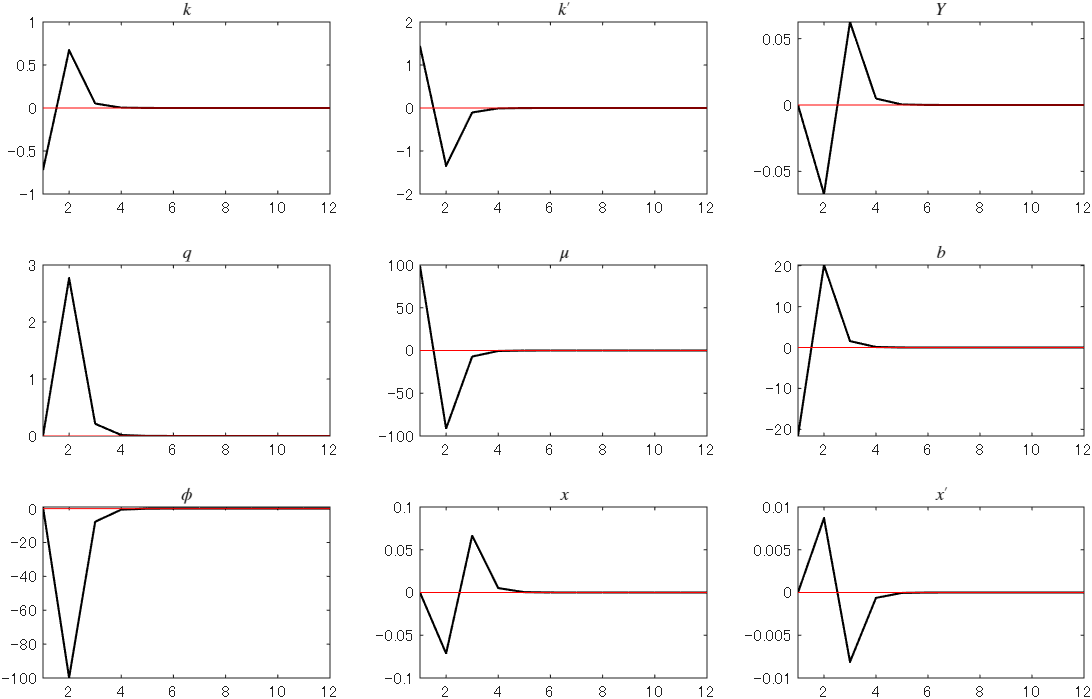
\includegraphics[scale=1.3]{5_2.png}
    \caption{Farmerの生産関数を$(a+c)k^\theta$に変更}
    \label{fig:5.2}
  \end{figure}
\end{landscape}

\subsection{総量規制ショックをFarmerの不動産保有$k$に対するショックとみなす（最終手段）} \label{k_change}
\begin{itemize}
  \item 当初想定していた総量規制ショックの導入方法である
  \item 総量規制は不動産投資を減少させる政策であるから，Farmerが所有する土地$k_t$に対する負のショックと捉える
  \item しかし，この$k$はFaemerの生産要素でもあることから，生産ショックと混じってしまい，ショックの識別戦略を考える必要がある
\end{itemize}

$k$に対する総量規制ショックを加えたモデルは以下のとおりである（生産ショックとの識別はできていない）
\begin{gather}
  k_t = \frac{((a+c)+q_t) k_{t-1} + b_t - \frac{b_{t-1}}{\beta'} - x_t}{q} (1+\varepsilon_t) \\
  b_t (1+\varepsilon_t) \leq \beta' q_{t+1} k_t \\
  x_t \geq c k_{t-1} \\
  1 + \varphi_t = (\beta(1+\varphi_{t+1}) + \mu_t) \frac{1}{\beta'} \label{} \\
  q_t (1 + \varphi_t) + \beta c \varphi_{t+1} = \beta(1 + \varphi_{t+1})[a + c + q_{t+1}] + \mu_t q_{t+1} \\
  q_t = \beta' [G'(k'_t) + q_{t+1}] \\
  x_t + m x'_t = (a + c) k_{t-1} + m G(k'_{t-1}) \\
  k_t = (\bar{K} - m k'_t) (1+\varepsilon_t)
\end{gather}

図\ref{fig:5.3}は，総量規制ショックをFarmerの不動産保有$k$に対するショックとみなした場合のIRF
\begin{itemize}
  \item 土地の総量は，$k_t + m k'_t = \bar{K}$で一定だから，$k_t$を減少させるショックは，$k'_t$を増加させる
  \item 借入金$b_t$，総生産量$Y_t$，不動産価格$q_t$のすべてが減少している
  \item 総じて，想定通りの動きをしていると言える
\end{itemize}

\newpage

\begin{landscape}
  \begin{figure}
    \centering
    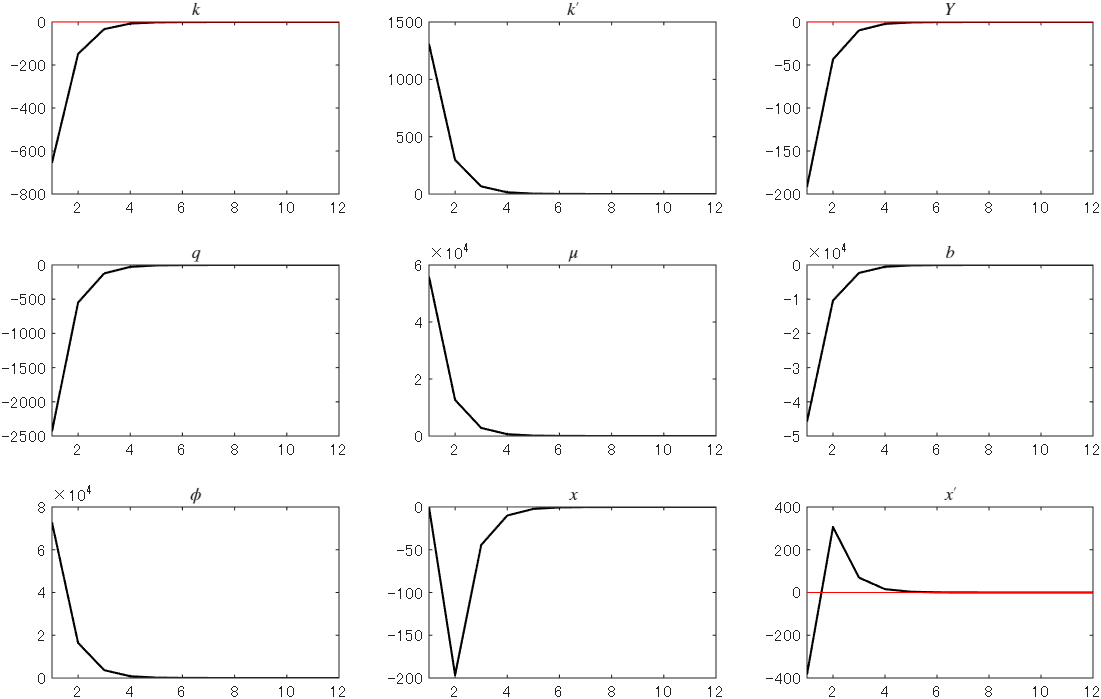
\includegraphics[scale=1.3]{5_3.png}
    \caption{総量規制ショックをFarmerの不動産保有$k$に対するショックとみなした場合}
    \label{fig:5.3}
  \end{figure}
\end{landscape}

\section*{付録}
\subsection*{\ref{q_change}節（借入制約の$q_{t+1}$を$q_t$に変更）のDynareコード}
\begin{lstlisting}
  var x, xp, b, k, kp, q, mu, phi, C, Y;
  varexo eps;
  parameters alpha, m, K_bar, beta, betap, a, c, z, theta;
  
  alpha = 1/3;
  m = 0.5;
  K_bar = 1;
  betap = 0.99;
  beta = 0.98;
  a = 0.7;
  c = 0.3;
  z = 0.01;
  
  model;
  [name='Euler equation bonds farmer']
  1 + phi = (beta*(1+phi(+1)) + mu)/betap;
  
  [name='Euler equation capital farmer']
  q*(1+phi) + beta*c*phi(+1) = beta*(1+phi(+1))*((a+c)+ q(+1)) + mu*q*(1-eps);
  
  [name='Budget constraint']
  q*(k - k(-1)) + b(-1)/betap + x = (a+c)*k(-1) + b;
  
  [name='Borrowing constraint']
  b = betap*q*k*(1-eps);
  
  [name='Euler equation gatherer']
  q = betap*(alpha*(z + kp)^(alpha-1) + q(+1));
  
  [name='Resource constraint']
  x + m*xp = (a+c)*k + m*(z + kp)^(alpha);
  
  [name='Capital market-clearing']
  k + m*kp = K_bar;
  
  [name='non-tradeable constraint']
  x = c*k(-1);
  
  [name='Aggregate consumption']
  C = x + m*xp;
  
  [name='Aggregate output']
  Y = C;  
  
  end;
  
  steady_state_model;
  q = a/(1-betap);
  kp = (betap*alpha/a)^(1/(1-alpha)) - z;
  k = K_bar - m*kp;
  b = betap*q*k;
  xp = (1/m)*(a*k + m*(z + kp)^(alpha));
  phi = (a*(beta-1) + beta*c)/(a*(1-beta));
  mu = (betap-beta)*beta*c/(a*(1-beta));
  x = c*k;
  C = x + m*xp;
  Y = C;
  end;
  
  shocks;
  var eps = 0.01;
  end;

  steady;
  check;

  stoch_simul(order=1, irf=12, Tex) k kp Y q mu b phi x xp;
\end{lstlisting}


\subsection*{\ref{product_change}節（Farmerの生産関数を$(a+c)k^\theta$に変更）のDynareコード}
\begin{lstlisting}[mathescape=true]
  var x, xp, b, k, kp, q, mu, phi, C, Y;
  varexo eps;
  parameters alpha, m, K_bar, beta, betap, a, c, z, theta;
  
  alpha = 0.05;
  m = 0.5;
  K_bar = 1;
  betap = 0.99;
  beta = 0.98;
  a = 0.3;  
  c = 0.1;
  z = 0.01;
  theta = 0.99;

  model;
    q * (k - k(-1)) + (1/betap) * b(-1) + x - c * k(-1)^theta = a * k(-1)^theta + b;
    b = betap * q(+1) * k * (1-eps);
    x = c * k(-1)^theta;
    1 + phi = (beta * (1 + phi(+1)) + mu) / betap;
    q * (1 + phi) + beta * c * phi(+1) * theta * k^(theta-1) = 
        beta * (1 + phi(+1)) * (theta * (a + c) * k(+1)^(theta-1) + q(+1)) + mu * q(+1) * (1-eps);
    q = betap * (alpha * (z + kp)^(alpha-1) + q(+1));
    x + m * xp = (a + c) * k(-1)^theta + m * (z + kp(-1))^alpha;
    k + m * kp = K_bar;
    C = x + m*xp;
    Y = C;
  end;

  initval;
    phi = (theta * beta * c) / (a * (1 - theta * beta)) - 1;
    mu  = (betap - beta) * (1 + phi);
  
    % k の「最初の推測値」として 0.5 を与える
    k = 0.5; 
  
    kp = (K_bar - k) / m;
    q = (a / (1 - betap)) * k^(theta - 1);
    b = betap * q * k;
    x = c * k^theta;
    xp = (a * k^theta) / m + (z + kp)^alpha;
  end;

  shocks;
    var eps = 0.01;
  end;

  steady;
  check;

  stoch_simul(order=1, irf=12, Tex) k kp Y q mu b phi x xp;
\end{lstlisting}

\subsection*{\ref{k_change}節（総量規制ショックをFarmerの不動産保有$k$に対するショックとみなした場合）のDynareコード}
\begin{lstlisting}
  var x, xp, b, k, kp, q, mu, phi, C, Y;
  varexo eps;
  parameters alpha, m, K_bar, beta, betap, a, c, z, theta;
  
  alpha = 0.05;
  m = 0.5;
  K_bar = 1;
  betap = 0.99;
  beta = 0.98;
  a = 0.3;  
  c = 0.1;
  z = 0.01;
  theta = 0.99;
  
  model;
    [name='Euler equation bonds farmer']
    1 + phi = (beta*(1+phi(+1)) + mu)/betap;
    
    [name='Euler equation capital farmer']
    q*(1+phi) + beta*c*phi(+1) = beta*(1+phi(+1))*((a+c)+ q(+1)) + mu*q(+1);
    
    [name='Budget constraint']
    k = (((a+c)+q)*k(-1) + b - b(-1)/betap - x)/q * (1-eps);
    
    [name='Borrowing constraint']
    b*(1-eps) = betap*q(+1)*k;
    
    [name='Euler equation gatherer']
    q = betap*(alpha*(z + kp)^(alpha-1) + q(+1));
    
    [name='Resource constraint']
    x + m*xp = (a+c)*k + m*(z + kp)^(alpha);
    
    [name='Capital market-clearing']
    k = (K_bar - m*kp)*(1-eps);
    
    [name='non-tradeable constraint']
    x = c*k(-1);
    
    [name='Aggregate consumption']
    C = x + m*xp;
    
    [name='Aggregate output']
    Y = C;
  end;
  
  steady_state_model;
    q = a/(1-betap);
    kp = (betap*alpha/a)^(1/(1-alpha)) - z;
    k = K_bar - m*kp;
    b = betap*q*k;
    xp = (1/m)*(a*k + m*(z + kp)^(alpha));
    phi = (a*(beta-1) + beta*c)/(a*(1-beta));
    mu = (betap-beta)*beta*c/(a*(1-beta));
    x = c*k;
    C = x + m*xp;
    Y = C;
  end;
  
  shocks;
  var eps = 0.01;
  end;
  
  resid;
  steady;
  
  stoch_simul(order=1,irf=12,ar=0,TeX) k kp Y q mu b phi x xp;
\end{lstlisting}



\end{document}








